\chapter{SPHERE-2 experiment}

\section{Method of reflected Cherenkov light to detect extensive air showers}

Cherenkov light is a valuable tool for studying extensive air showers (EAS) due to its weak dependence on high-energy hadronic interaction models. The traditional direct detection method, similar to charged particle detection, employs ground array of detectors distributed over a large area to point-measure flux density.

However, unlike charged particles, Cherenkov light in the optical and near-optical range can be effectively scattered by the Earth's (for example, snow) surface and observed from above. The method of registering reflected light was first proposed by A. E. Chudakov \cite{Chudakov1972} and further developed in the SPHERE-1 and SPHERE-2 experiments \cite{Antonov1997, Antonov2001}.

One of the main advantages of this method is the access to Cherenkov light from the paraxial region of the shower, made possible by the extended fields of view of individual sensitive elements of the detector.

\section{SPHERE-2 detector}
\label{sec:sphere-2-model}

\subsection{Geometry}
\label{sec:light-collection-from-surface}

The SPHERE-2 detector was lifted by a balloon and suspended at an altitude ranging from $400$ to $900~\text{m}$. It utilized an optical system comprising a diaphragm, a spherical mirror, and a mosaic of photomultiplier tubes (PMTs) to collect Cherenkov light from EAS reflected by the snow surface below. Each PMT collected reflected light from an area with a diameter ranging from $10$ to $50~\text{m}$, depending on the detector altitude. Figure \ref{pic:sphere-detector-optical-scheme} illustrates the optical scheme of the SPHERE-2 detector.

\begin{figure}
	\centering
	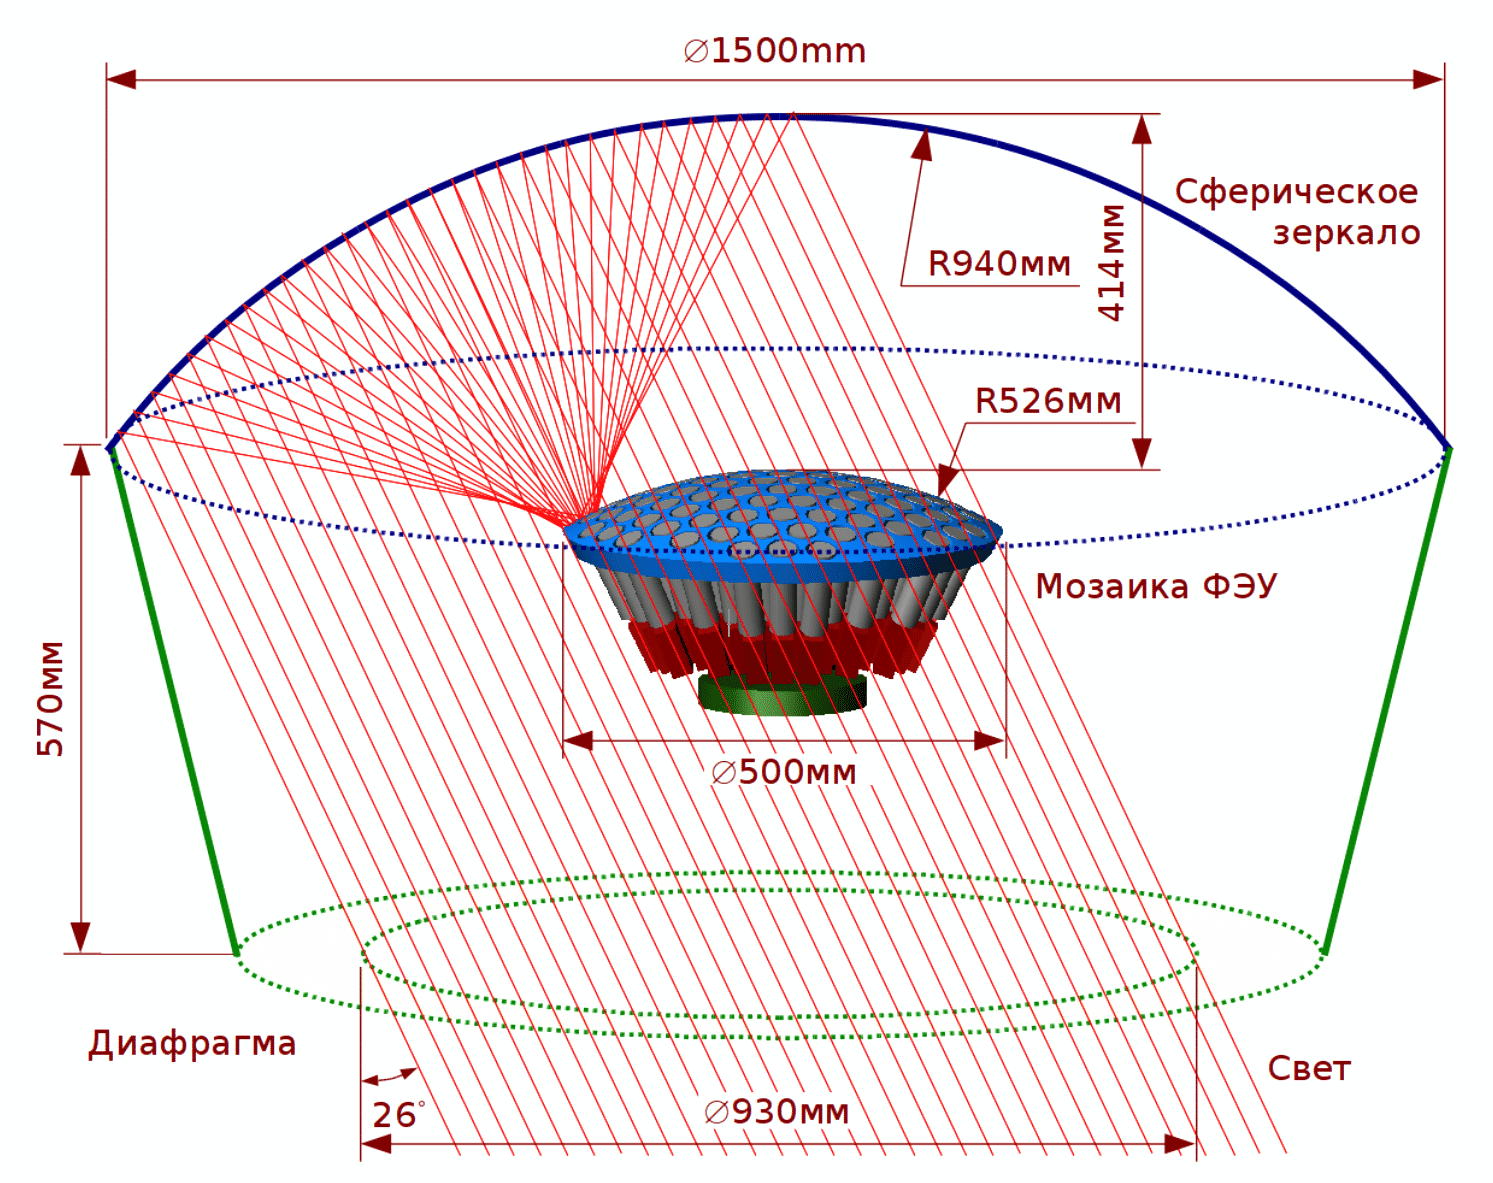
\includegraphics[width=0.9\columnwidth]{optical_scheme}
	\caption{SPHERE-2 detector optical scheme}
	\label{pic:sphere-detector-optical-scheme}
\end{figure}

The PMT mosaic, arranged in an approximately hexagonal grid, was located near the focal surface of the spherical mirror. It consisted of 109 PMTs, with the central PMT being the Hamamatsu R3886, serving as a reference for detector calibration \cite{SphereCalibration2016}, and the remaining PMTs being Soviet-made PMT 84-3.

\subsection{Intermediate PMT mode}
\label{sec:photon-to-phels-conversion}

When light strikes the PMT photocathode, it emits a photoelectron with a certain probability. This photoelectron then triggers a cascade of secondary photoelectrons through the dynode system, resulting in an observable charge at the anode.

The electron cascade within a PMT is a fundamentally stochastic process, as verified by direct laboratory measurements of anode charge fluctuations \cite[Fig. 9]{SphereCalibration2016}. Each dynode undergoes random multiplication, and due to the cascading nature, small variations in the early stages can lead to significant differences in amplification.

The stochastic nature of PMT amplification is not apparent when measuring high fluxes due to averaging. Likewise, it is not significant at low fluxes when the PMT operates in photon counting mode, allowing for the observation of well-resolved individual pulses. However, in the SPHERE-2 detector, PMTs operate in an intermediate mode: the flux is too high to resolve individual photons, yet insufficient for effective averaging. Consequently, the deconvolution problem needs to be formulated in statistical terms.